\documentclass{beamer}
\usepackage[utf8]{inputenc}
\usepackage{amsmath}
\usepackage{amsthm}
\usepackage{algorithm}
\usepackage{algorithmic}
%% Sets page size and margins
%\usepackage[a4paper,top=3cm,bottom=2cm,left=3cm,right=3cm,marginparwidth=1.75cm]{geometry}
\DeclareMathOperator*{\argmax}{arg\,max}
\DeclareMathOperator*{\argmin}{arg\,min}
% \DeclareMathOperator*{\max}{max}
% \DeclareMathOperator*{\min}{min}
\usepackage{graphicx}
\usepackage{amsfonts,amssymb}

\title{Variational Calculus}
\author{}
\date{June 2019}

\begin{document}

\maketitle

\begin{frame}{Intro to infinite-dimensional optimization}
    \begin{figure}
        \centering
        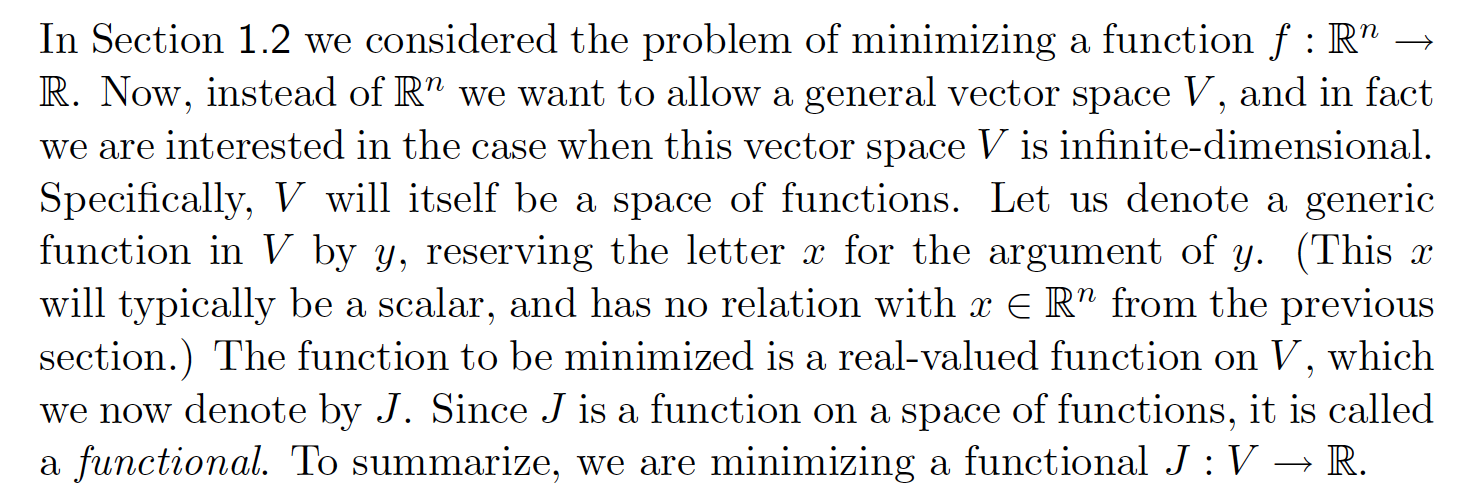
\includegraphics[width=\linewidth]{ch1/fig1.png}
    \end{figure}
\end{frame}

\begin{frame}{Norms for function spaces}
    \begin{itemize}
        \item We will frequently work with the function space $V = \mathcal{C}^k([a,b], \mathbb{R}^n)$ whose elements are k-times differentiable.
        \item The two norms that we will be focusing on are
        \begin{itemize}
            \item 0-norm: 
            \begin{equation}
                \Vert y \Vert_0 = \max_{a \leq x \leq b} \vert y(x) \vert
            \end{equation}
            $y \in V$ and $\vert \cdot \vert$ is just the euclidean norm.
            \item 1-norm: 
            \begin{equation}
                \Vert y \Vert_1 = \max_{a \leq x \leq b} \vert y(x) \vert + \max_{a \leq x \leq b} \vert y'(x) \vert 
            \end{equation}
            $y \in V$ and $\vert \cdot \vert$ is just the euclidean norm.
        \end{itemize}
    \end{itemize}
\end{frame}

\begin{frame}{Local minima of a functional}
    \begin{figure}
        \centering
        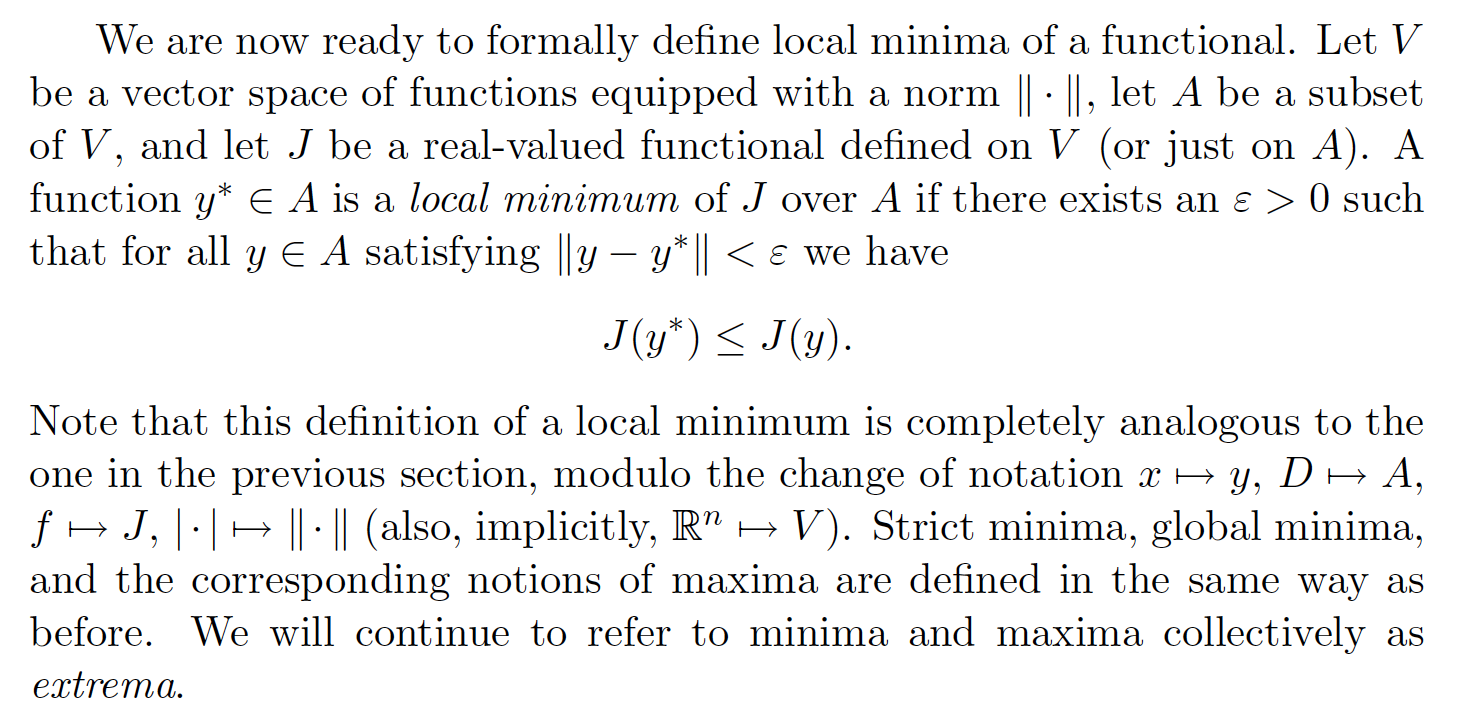
\includegraphics[width=\linewidth]{ch1/fig2.png}
    \end{figure}
\end{frame}

\begin{frame}{First variation}
     \begin{figure}
        \centering
        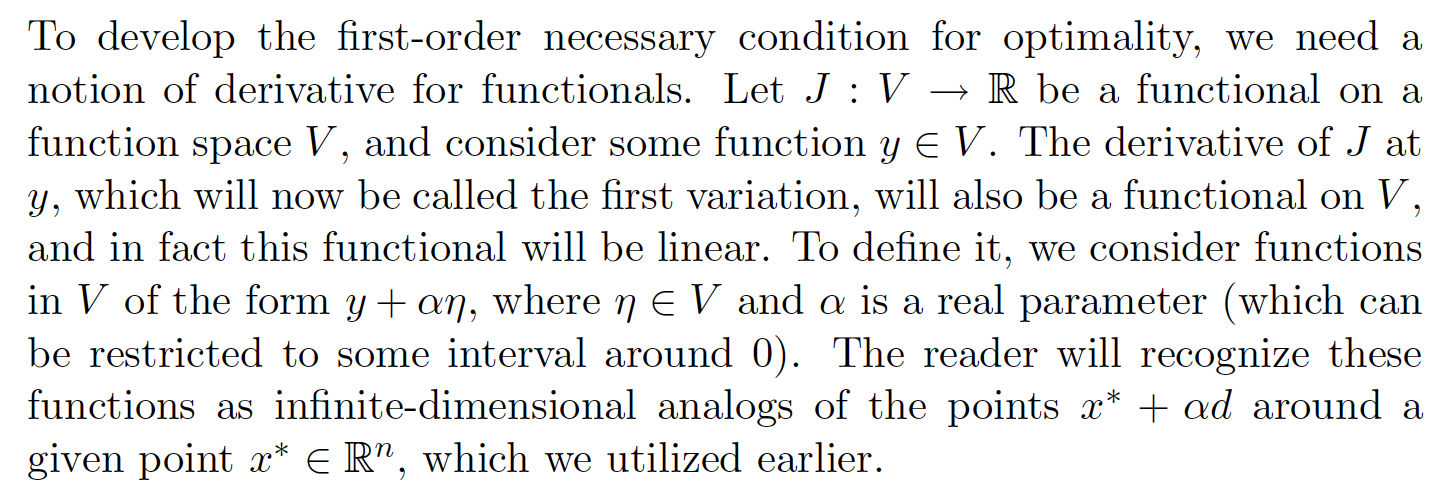
\includegraphics[width=\linewidth]{ch1/fig3.png}
    \end{figure}
\end{frame}

\begin{frame}{First variation}
    \begin{figure}
        \centering
        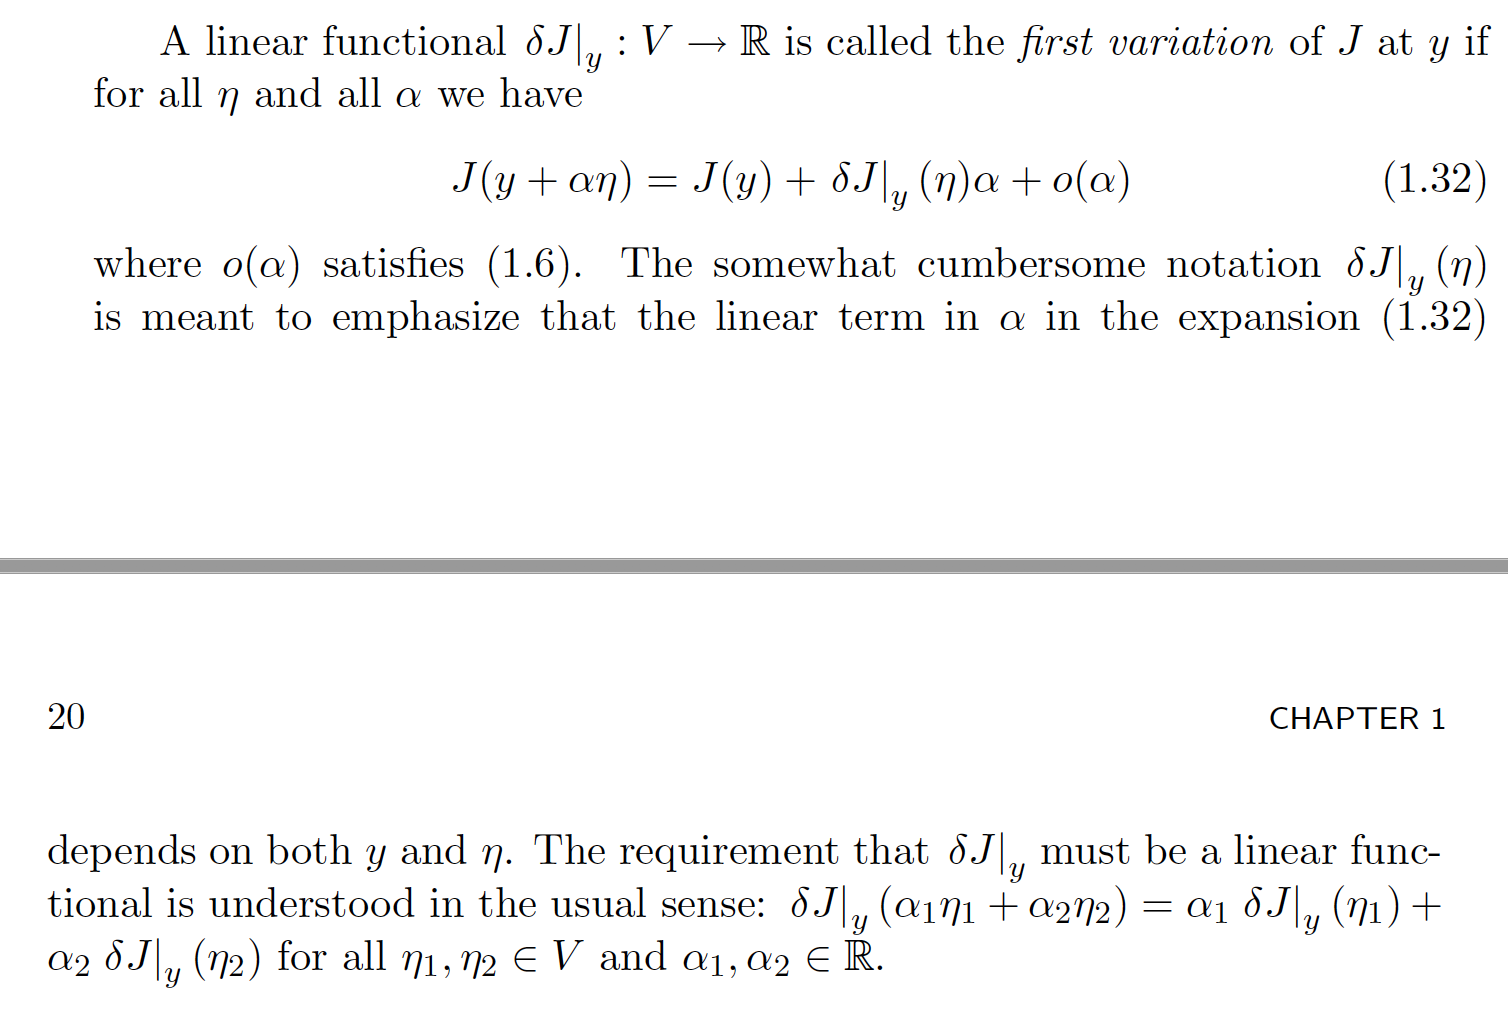
\includegraphics[width=\linewidth]{ch1/fig4.png}
    \end{figure}
\end{frame}

\begin{frame}{First variation}
    \begin{figure}
        \centering
        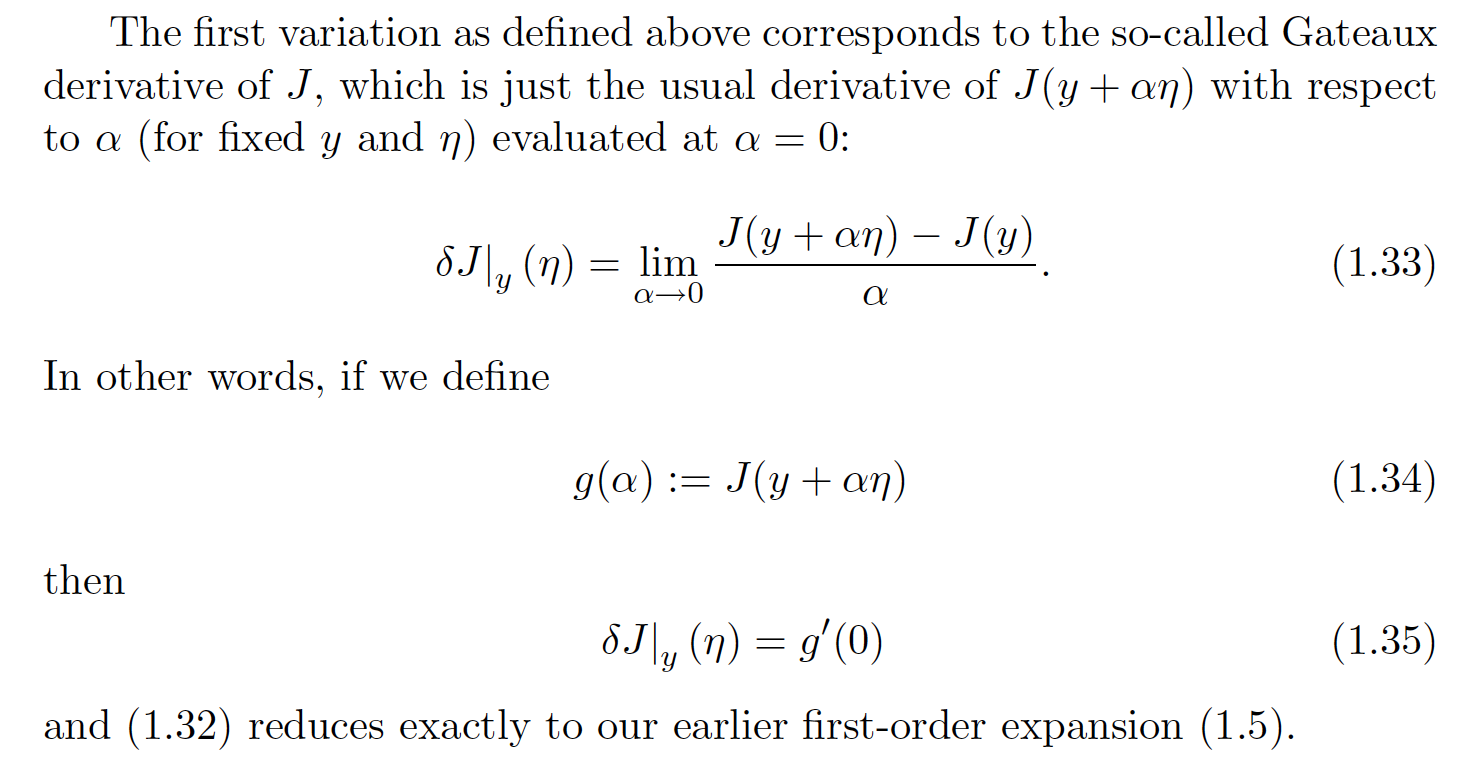
\includegraphics[width=\linewidth]{ch1/fig5.png}
    \end{figure}
\end{frame}


\begin{frame}{First-order necessary condition}
    \begin{itemize}
        \item Now, suppose that $y^*$ is a local min of J over some subset $A$ of $V$.
        \item $\eta \in V$ is a perturbation which will be commonly used throughout the book.
        \item $\eta$ is an admissible perturbation if $y + \alpha \eta \in A$ for $\alpha$ close to 0.
        \item By the same logic used in finite-dimensional optimization, we get to the \textbf{first-order necessary condition for optimality}: \textit{$\delta J \vert_{y^*} (\eta) = 0$ for all admissible perturbations, $\eta$}.
    \end{itemize}
\end{frame}

\begin{frame}{Basic calculus of variations problem}
\begin{itemize}
    \item Consider a function $L: \mathbb{R} \times \mathbb{R}^n \times \mathbb{R}^n \rightarrow \mathbb{R}$
    \item Among all $\mathcal{C}^1$ curves $y:[a, b] \rightarrow \mathbb{R}^n$ satisfying given boundary conditions
    \begin{equation}
        y(a) = y_0, \quad y(b) = y_1
    \end{equation}
    find the (local) minima of the cost functional
    \begin{equation}
        J(y) = \int_a^b L(x, y(x), y'(x))dx
    \end{equation}
    \item L is called the \textit{Lagrangian} or \textit{running cost}.
    \item Important: Even though $y$ and $y'$ are dependent, L is to be viewed as a function of three independent variables!
\end{itemize}
\end{frame}

\begin{frame}{Weak and Strong Extrema}
\begin{figure}
        \centering
        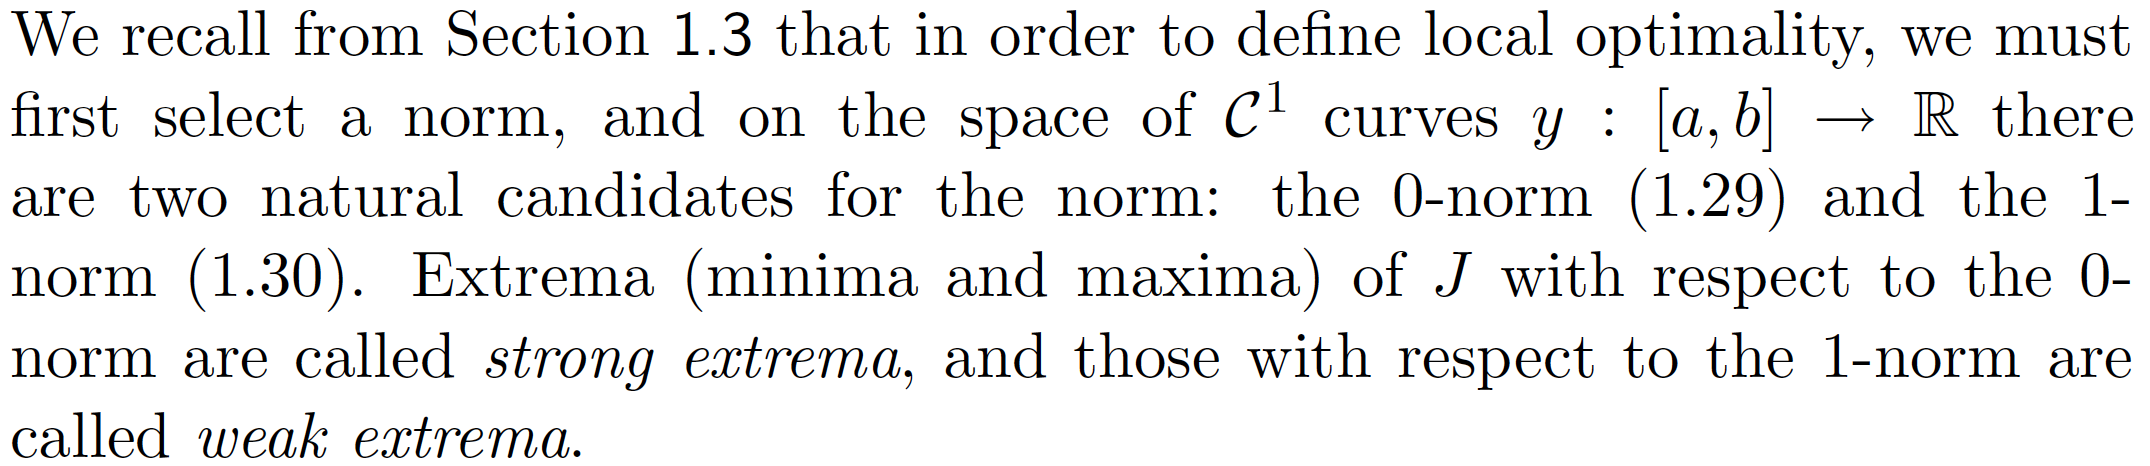
\includegraphics[width=\linewidth]{ch2/fig7.png}
    \end{figure}
\end{frame}
\end{document}
